\chapter{Validation \& Experiments}


using login because it is be able to sign in immediately 
\begin{verbatim*}
"C:\tools\chromedriver.exe" "1920x900+0+0" "http://localhost:8100/Login"
\end{verbatim*}

To prevent the system to logout it is needed to filter the logout action, \verb|.*Logout.*| added to the filter option. 

\begin{lstlisting}[language=Java, caption=Begin Sequence code, label=code:beginSequence]
@Override
protected void beginSequence(SUT system, State state) {
	super.beginSequence(system, state);

	waitLeftClickAndPasteIntoWidgetWithMatchingTag("id", "url", "http://localhost:5000", state, system, 5,1.0);
	waitLeftClickAndTypeIntoWidgetWithMatchingTag("id","username", "testar2\\testar", state, system, 5,1.0);
	waitLeftClickAndTypeIntoWidgetWithMatchingTag("id","password", "testar", state, system, 5,1.0);
	waitAndLeftClickWidgetWithMatchingTag("name", "Sign In", state, system, 5, 1.0);
}
\end{lstlisting}



\section{Gherkin style testing}
The first form of validation the algorithm is done with Gherkin syntax testing. Gherkin is syntax that describes a test scenario. The syntax uses special keywords like \textbf{Given}, \textbf{When}, \textbf{Then} to describe a \textit{scenario}. An example of a Gherkin scenario can be found in listing \ref{code:gherkin-example}.

\begin{lstlisting}[language=Gherkin, caption=Calculator test example, label=code:gherkin-example]
Scenario: Add two numbers
Given the first number is 50
And the second number is 70
When the two numbers are added
Then the result should be 120
\end{lstlisting}

A developer can automated the Gherkin syntax to create automated test cases for example with the help of Specflow \footnote{\url{https://www.specflow.com}}. Specflow is a test automation solution for the .NET framework \cite{specflow}. The code to automate the 'then' line in listing \ref{code:gherkin-example} can be implemented as indicated in listing \ref{code:gherkin-example-code}.

\begin{lstlisting}[language=Java, caption=Implementation of a 'then' line, label=code:gherkin-example-code]
[Then("the result should be (.*)")]
public void ThenTheResultShouldBe(int expectedResult)
{
    Assert.AreEqual(expectedResult, actualResult);
}
\end{lstlisting}

To validate the algorithm and the merging of the two abstract models (see \ref{sec:merge-graph}) a couple of scenario are written. The scenario's can be found in appendix \ref{appendix:test-scenarios}. The file start with the keyword \textbf{Feature} which is Specflow solution to group scenario's together. The \textbf{Background} section generates four in-memory graphs. In figure \ref{fig:test-graphs} the four graphs are displayed. 

\begingroup
\captionsetup{type=figure}
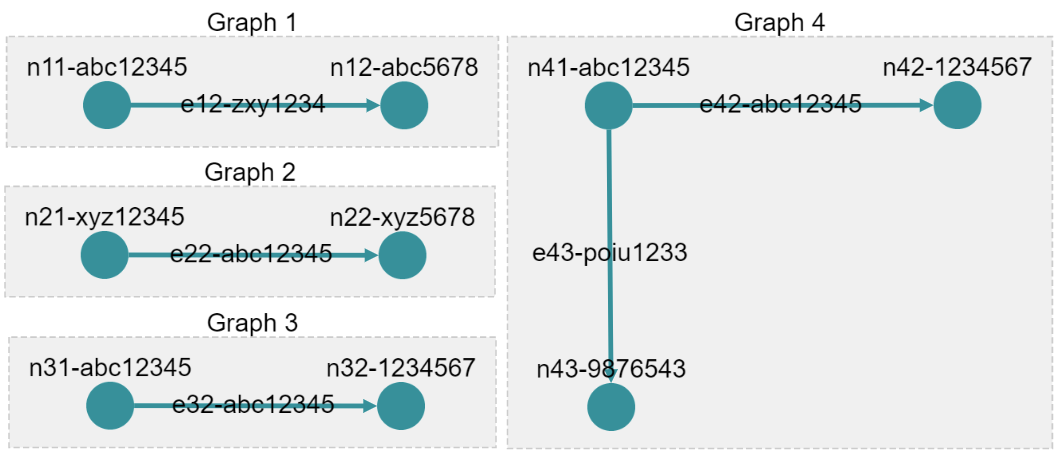
\includegraphics[scale=0.6]{images/6-TestGraphs.png}
\captionof{figure}{Test graphs used for testing. The circle represents a abstract state, the line represents the abstract actions between the abstract states}\label{fig:test-graphs}
\endgroup

\begingroup
\captionsetup{type=figure}
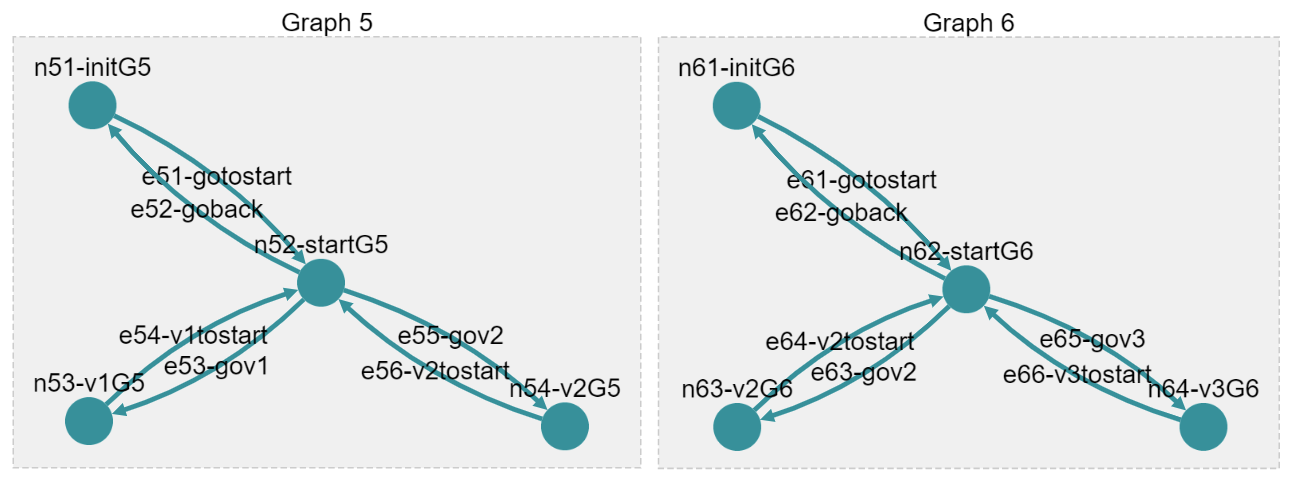
\includegraphics[scale=0.5]{images/6-test-graph-5-6.png}
\captionof{figure}{Graph 5 and 6 for bigger scenario. The circle represents a abstract state, the line represents the abstract actions between the abstract states}\label{fig:test-graphs}
\endgroup